%!TEX root = ../main.tex
\chapter{An Unified Efficient Particle Physics Framework}
\label{new_lipmini}

Programming for homogeneous platforms poses a series of challenges not faced when coding parallel applications due to the shared memory paradigm. In this context, the data is always easily accessible when coding, as the different memory bank accesses are managed by the compiler and hardware. Data dependencies and races still need to be managed by the programmer, which may required a significant level of expertise. To efficiently use the computational resources, dealing with problems such as false sharing or efficient cache usage, the programmer must have an advanced expertise on both the coding and architectural details of homogeneous platforms.

Since an heterogeneous platform is a distributed memory environment, where the CPUs shared the memory with each other but not with the hardware accelerators, a series of new challenges arise. All communications of data between CPU and accelerator must be explicitly coded by the programmer, and has an added latency associated. The balance of the work for each computing device to process becomes harder as it must take into account the data transfers and different characteristics of the devices.

Each different hardware accelerator has its own architectural design principles, as show in section \ref{hardware}, which constrain the way they are programmed and the characteristics that both the algorithm and the code must have to efficiently use the computational resources. This implies that the programmer must be able to learn the hardware intrinsic characteristics and adapt to a new programming paradigm. Even for experienced programmers, adapting current applications to run on heterogeneous platforms may be infeasible without redesigning all major algorithms, as opposed to code a new application specifically for these platforms. This issue has an higher impact on legacy code.

Scientists are usually self-taught programmers that only consider coding as a necessary tool to perform their research. Several studies, referred in section \ref{motivation}, identified a set of problems with scientists coding practices and scientific computing. Most of their code is in constant development, up to decades long, only adding or changing functionalities in each iteration, not considering any software engineering principles and not adapting the code to the changes in hardware. The few that worry about performance attempt to address the code regions that they think are the bottleneck, not knowing of the existence of profiling tools and even compiler optimisations.

Since most scientists develop applications with the help of specialised frameworks of their research field, they expect them to be efficient, by resorting to parallelisation or other techniques. However, the bottleneck is often on the scientists code rather than in the framework, and these tools are not designed to automatically extract parallelism from their code.

Scientists usually do not have any training for programming efficient applications for homogeneous systems or cluster environments, as programming is just a necessity for their field of research. They are even more reluctant to learn the new programming paradigms required to work with hardware accelerators on heterogeneous platforms. With this in mind, several automatically parallelisation frameworks for these systems were developed by computer scientists, as presented in subsection \ref{distributed_mem}.

These general purpose frameworks usually have a steep learning curve, even for computer scientists. One significant setback of these frameworks is that, even if it is not explicitly required, the application must be designed to the framework characteristics, rather than the framework adapt to the application. As scientists are usually reluctant to redesign the very complex legacy code, which is difficult for computer scientists to understand without the expertise of the science field, an integration with these frameworks is infeasible. This problem also applies to the most of the external libraries used by these applications, as their functions are not coded to run on hardware accelerators and adapting the source code may not be possible.

Even though, scientists are not willing to endure the steep learning curve of these frameworks to integrate with future applications, and do not want to code two versions of the core algorithms to run on the CPU and accelerator. Their complexity and the lack of guarantees to that they will increase the code performance, due to poor implementation or algorithm characteristics, puts the scientists further away from these frameworks. Also, they attempt to have few dependencies of an application with external libraries, as the external tools are not guaranteed to be supported through the application lifetime.

The existence of general purpose automatically parallelisation frameworks is useful, specially for computer scientists, but the scientific community lacks frameworks that both address the intrinsics of their scientific field, in which scientists can trust and rely, and the efficient usage of the computational resources, on both homogeneous and heterogeneous platforms. Frameworks such as these sacrifice the abstraction to interact with any scientific field, but are more adapted to the scientific problem that is addressed. A lower abstraction level leads to an easy interaction of the scientist with the tool (and even abstract them of any parallelisation complexities) and increases the computational efficiency of the code when compared with general purpose frameworks, as the main bottlenecks are usually known \textit{a priori} and the framework is designed around their characteristics. The development of such frameworks may lead to a better interface of computer scientists and researchers, causing and improvement of their codes with the implementation of software engineering concept, increasing the quality of the research.

\section{The LipMiniAnalysis Skeleton Library}
\label{lipminianalysis}

The LipCbrAnalysis was a skeleton developed by two researchers of LIP in 2005, with the purpose of aiding the development of data analysis applications within the research group. Initially it served as an interface for dealing with the I/O of the data, transforming it from the format supported by ROOT at the time to variables in the global memory of the skeleton. All other standard functions needed for the analysis had their prototypes declared, but it was the programmers job to code them to his needs, knowing that the required data for each event was on memory.

Along the years the code was successively iterated to add support for new data file formats, physics functionalities, and general features, such as the support for passing options and arguments to the executable. Some of the functions that the programmer needed to code were now fully implemented, with the option of being override by the user.

The LipMiniAnalysis is the latest development iteration on a production environment. It discarded outdated features that were no longer necessary, and reads the new Mini Ntuple data format, hence its name. It is not a standard ROOT data format, but rather a set of events that suffered some preprocessing to improve the quality of the data and filter events that do not show any interesting physics.

Figure \ref{fig:lipmini} presents the structure of LipMiniAnalysis, where all sections marked with a \textbf{*} need to be coded by the programmer. When the application starts it sets the default values for all control information needed by the event filtering and reconstruction. The \textit{Set User Values} section allows for the user to set its own control parameters, for both information defined by \textit{Set Default Values}, overwriting the existing configuration, and parameters not set yet. The \textit{Get Command Line Options} section is responsible for defining and interpreting the options defined by the user when starting the executable. It is partially defined with standard options for every analysis, such as the definition of the systematics file and output directory, but the programmer can add new options as needed. The systematics parameters are automatically configured based on the input systematics file, so no user interaction is necessary. The preparation of both the input and output files is done automatically, but the declaration of the histogram vectors must be coded by the programmer, as it depends on the event type, filtering and reconstruction techniques applied.

\begin{figure}[!htp]
	\begin{center}
		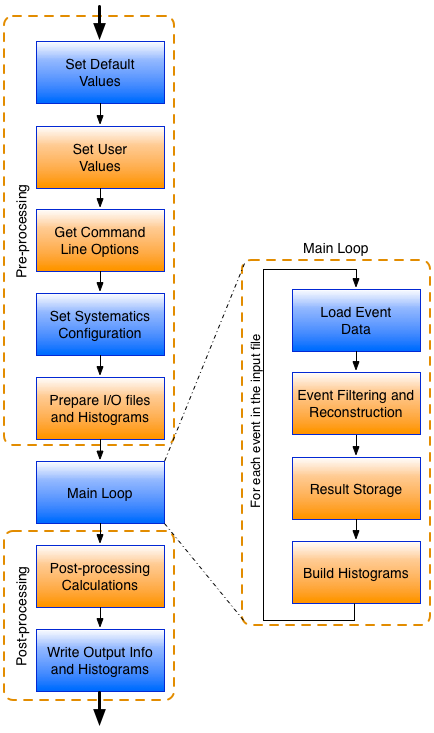
\includegraphics[scale=0.5]{imgs/lipminianalysis.png}
		\caption{Schematic representation of the LipMiniAnalysis skeleton structure. The \textbf{*} mark represents the sections of the skeleton that the programmer must code.}
		\label{fig:lipmini}
	\end{center}
\end{figure}

The \textit{Main Loop} is responsible for individually loading an event from the input file, apply the filters, reconstruct it if it passes the required filters, store the results, and build the histograms for each filter and final reconstruction. Only the event loading is automatic, so the programmer must code all remaining sections, as they vary among different analysis. The final post-processing also depends on the analysis, so it is not coded. Then, LipMiniAnalysis automatically writes all output information. Note that this is a logical structure of the code; in the current implementation most features are not properly organised and LipMiniAnalysis would have great benefits from a reorganisation of its structure, code-wise.

Studies presented in \cite{Msc:AMP,paperAMP} targeted the computational efficiency issues of a specific data analysis application of LIP, related to the reconstruction of the \ttH system. This data analysis was developed using the LipMiniAnalysis and, although the goal was to address only the inefficiencies of the data analysis itself, problems with the main data structure of the skeleton restricted the performance scalability, specially on heterogeneous platforms.

The LipMiniAnalysis was designed to store only one event in the application global memory for the \textit{Main Loop} to load and process. The data for an event is composed of hundreds of variables, from simple scalars to complex vectors of ROOT classes. With only a single event in memory, it is more difficult to create an efficient parallelisation with only the event reconstruction tasks, due to the low amount of work to balance, specially on distributed memory environments as it will require more communications through the application lifetime. With all events from an input data file on the application global memory, a more efficient parallelisation for both shared and distributed memory systems can be achieved. It would also help the implementation of automatic parallelisation in LipMiniAnalysis.

\section{The Proposed Framework}
\label{new_framework}

A physics framework to replace LipMiniAnalysis in aiding the development of data analysis applications is proposed. Its design and specification will include several software engineering concepts to provide a stable and robust tool that will increase the researchers productivity, spending less time coding and more time analysing data and improving physics algorithms, and ensure the generation of efficient data analysis applications by automatically parallelising the code. It will include both redesigned features of LipMiniAnalysis and new physics functionalities.

Improving both the researcher coding productivity and data analysis computational efficiency has a direct impact on the research quality. To achieve this goal, the proposed framework has to utilise the capabilities of modern computing systems and software. This implies that the LipMiniAnalysis code design, based on the LipCbrAnalysis developed in 2005, does not suit the characteristics of current hardware. The new framework will implement all required features present in LipMiniAnalysis but designed to modern specifications of hardware, software, and modularity to interact with new features.

Figure \ref{fig:new_framework} presents the organisation and dependencies of the different modules of the proposed framework. A modular organisation and implementation allows for the framework to be robust and easily extensible in the future. The \textit{Physics} and \textit{Histograming} modules will be implemented using redesigned features currently available at LipMiniAnalysis, as they have standard features used by most data analysis applications. The framework will have to support both ROOT and TopROOTCore libraries without any specific configuration by the user. TopROOTCore installation with the framework may be an option to the user, since only a part of event data analysis applications use its functionalities, which are more useful for data preparation.

\begin{figure}[!htp]
	\begin{center}
		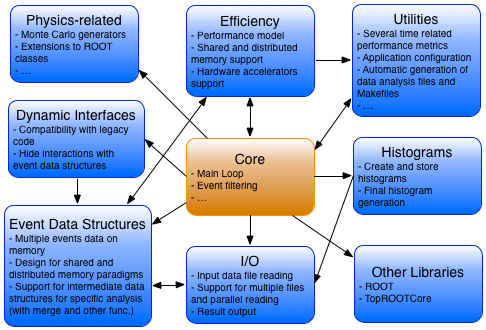
\includegraphics[scale=0.7]{imgs/new_framework.png}
		\caption{Schematic representation of the proposed framework modules and their dependencies.}
		\label{fig:new_framework}
	\end{center}
\end{figure}

The \textit{I/O} module is responsible for loading the input data files for processing the events in the data analysis applications. The LipMiniAnalysis reads only MiniNtuples, which are preprocessed events at the previous computational tiers, which are used by some applications, but other file formats may also be supported, as requested by researchers. Different file formats have different structures and auxiliary event parameters stored, although the core event information is similar. The file reading must support parallel file descriptors, so that it is possible that each thread/process reads its own event data, reducing the communications cost and initial load distribution overhead.

The \textit{Event Data Structures} module will be dependent on the file type to be read. Its purpose is to have a C++ class, or set of classes, to hold all the information of an event on memory in a structured way, opposed to the current implementation on LipMiniAnalysis. Then, it must hold a STL collection (vector, map, etc) to store the instantiations of the event class, enclosing all events in the input data file. An assessment of the different file formats used at LIP will be required to evaluated the benefits of having a single abstract event class or specific classes for each file format. Both the event class design and storing collection must be suitable for both shared and distributed memory parallelisation, with good performance for data structure splits (to balance the load, specifically in distributed memory paradigms), transverses (to iterate through the events on each split segment), and low overhead (un)marshalling computations for communicating the data. The module may also contain specific data structures for intermediate processing, as explained in detail in subsection \ref{work_so_far}, suitable to run on hardware accelerators, considering the limitations that they incur.

The \textit{Dynamic Interfaces} module will hold the interface generator and respective interfaces for each different event data structure. Its purpose is to make the framework compatible with legacy code, allowing for current data analysis to benefit from the automatic parallelisation and improved efficiency of the proposed framework. Also, it must hide the interaction of the user with the data structures, to provide a simpler programming interface, later explained in more detail. Since there may be several different data structures, and their code may be changed periodically, the interface generator must be capable of parsing the data structure source files and dynamically generate the interfaces.

The \textit{Utilities} module implements several auxiliary features usable in both the framework and data analysis code. It will have simple performance statistics, such as execution time of the application, communications time, event processing throughput, etc. A more robust command line options reader will be available, with all required options for executing all different data analysis, which can be extended by experienced users.

The \textit{Efficiency} module will have all necessary functionality required to create parallel tasks and manage the load distribution for both homogeneous and heterogeneous platforms with hardware accelerators. The performance model must be capable of assessing if an hybrid multithreaded process parallelisation provides better efficiency than a simple implementation, which was proven to happen in some data analysis \cite{paperAMP}. There is no automatic parallelisation tool that attempts hybrid implementations such as this, only opting for a shared or distributed memory paradigm (usually the last is only used when the hardware forces to) and uses an efficient amount of parallel tasks, but it may prove beneficial to have this mix of processes and threads in some specific cases. This might require an higher overhead to obtain the best process/thread configuration, but since these data analysis run for several hours the initial setup cost is minimum. It also can produce a configuration file when the configuration is performed for a given data analysis on a given computing system, which can avoid performing the initial setup every time the application is executed.

This module must also be able to assess, with some help of the user, what sections of the data analysis code can be executed in the hardware accelerators, and if it has the required characteristics to efficiently use these devices. While this might seem complex for general purpose parallelisation frameworks, dealing with only a specific problem such as physics data analysis applications helps the design of the performance model around these features. Implementation-wise, these features require heavy modifications to current automatic parallelisation frameworks. However, a new implementation designed to this specific problem, with components adapted from current frameworks, may provide a better and more simple integration and performance efficiency of data analysis applications.

The \textit{Core} module will integrate all previous modules, implementing the major routines responsible for the event analysis, ranging from the filtering to the final output data storage. It will have assembled all the specific bits of each module to process the events, as well as the code sections that is for the user to code. Note that the user will not edit the code in the framework, but rather on the data analysis source code that will later link the missing parts into the framework.

Features that are very important for the most compute intensive sections of data analysis applications will be implemented to run on CPU and accelerator devices. These features will be provided in the framework API. For example, when selecting an pseudo-random number generator to use in a compute intensive section, such as the event reconstruction, the user must avoid the \texttt{TRandom} available in ROOT and use the one provided by the framework. The framework compiles the code to run on CPU, which uses \texttt{TRandom}, and on GPU, which uses the \texttt{cuRand} (with the same PRNG algorithm). This only applies for features that produce the same result on any computing accelerator. Otherwise, an alternative is suggested for each computing device that the user may chose to accept.

\subsection{Usage and Workflow}
\label{usage_workflow}

One of the goals of the framework is to provide a kernel-like programming model to the user, with as minimum interaction as possible. This eases the development of new data analysis applications and increases their portability. Once the framework is installed on a system, the user just needs to copy their code and it is expected to compile, as all external dependencies are handled by the framework. Its flow is presented in figure \ref{fig:new_framework_flow}. Note that LipMiniAnalysis, presented in section \ref{lipminianalysis}, has a similar logical structure, but it does not reflect the code organisation and structure. In the new framework, the code will follow this structure to improve its modularity and reliability.

\begin{figure}[!htp]
	\begin{center}
		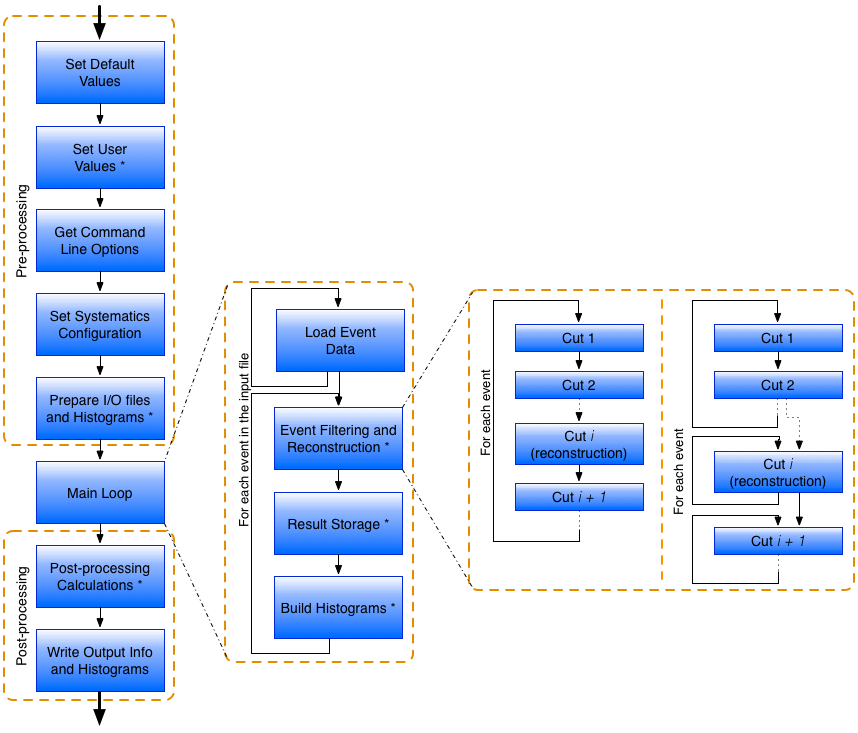
\includegraphics[scale=0.5]{imgs/new_framework_flow.png}
		\caption{Schematic representation of the proposed framework flow. The \textbf{*} mark represents the sections of the workflow coded by the programmer.}
		\label{fig:new_framework_flow}
	\end{center}
\end{figure}

The user intervention is required at four stages of the event processing (implementation-wise, the \textit{Result Storage} and \textit{Build Histograms} are coded together as \textit{Filter Post-process}). The data analysis is expected to be implemented as a class, which will extend the \texttt{DataAnalysis} class provided by the framework, and must contain at least a set of predefined methods that represent each of the stages that the user must code. The coding is very intuitive, as the user must implement the set of features required to process a single event, in the logical pipeline reasoning. The user does not interact directly with the event data structure, but through the respective interface, which gives the illusion that only a single event is on memory, as physicists were used to program. The framework will be responsible for applying the code in parallel to all events on memory, not necessarily following the pipeline order but respecting the dependencies.

The data analysis stages are characterised as follows:

\begin{description}
	\item[\textit{User Setup}:] this is only executed at the beginning of the data analysis execution, where the user specifies the initial \textit{User Values}, as in the LipMiniAnalysis flow, output files, and histogram configurations. The user can also easily specify any additional parameters to read by both command line and environment variables, using the respective framework utilities, and a small set of configurations to help the parallelisation setup.
	\item[\textit{Event Filtering and Reconstruction}:] this holds the code required to filter and reconstruct a single event. As shown in figure \ref{fig:new_framework_flow}, two templates are provided. The first is the traditional pipeline for the event processing, oriented for novice users. The second provides three sections: pre-filtering, reconstruction, and post-filtering. The user codes in the pre-filtering the filters applied before the reconstruction, the reconstruction, and then the final filters (if applicable), in three separate methods. This is useful when the reconstruction takes most of the execution time and this provides more parallelism (as it is applied simultaneously to all events) and better load management, specially when using heterogeneous platforms.
	\item[\textit{Result Storage} and \textit{Build Histograms}:] this is coded as a single method, since both operations are closely dependent in most implementations. The user store the results of the previous filtering to later be printed in the output file.
	\item[\textit{Post-processing Calculations}:] this stage is executed once, after processing all events. The user codes all final calculations before the results and histograms output.
\end{description}

Note that this design of the stages required by the \texttt{DataAnalysis} class will be changed after the requirements elicitation and an usability study with the LIP researchers. All major features are initial design and testing is performed in close cooperation with a subset of LIP physicists, working on top quark and Higgs boson research.

However, the programmer will have some guidelines to avoid producing an inefficient data analysis. Class variables in \texttt{DataAnalysis} must be avoided because of the amount of communications required to maintain the consistency and coherence of that data on a distributed memory environment. To maintain portability, the data analysis must only depend on the libraries provided by the framework (at the moment, there is none data analysis in LIP that depends on other libraries). To run on heterogeneous platforms, the analysis critical region must only depend on features that the framework has implemented for both CPU and accelerator devices. This allow for the user to code the data analysis once and the critical regions are able to execute on any computing device. Otherwise, the code will be restricted to the device that can execute it.

\subsection{Preliminary Prototypes}
\label{work_so_far}

Some of the work towards the creation of the new framework was already developed. These prototypes were integrated and tested with the current version of LipMiniAnalysis using the \ttH data analysis application presented in \ref{ttH}, but have a modular design to be properly merged into the final framework, and they may suffer structure or implementation changes throughout its development. Proposed prototypes for several features required by the framework are presented next.

\subsubsection*{A new event data structure}

The information of an event is loaded in the \textit{Main Loop} into a single global memory state. The hundreds of variables of an event are spread among a set of files of LipMiniAnalysis. To create a new event data structure all these variables must be merged into a single C++ class, which represents a single event, named \textit{EventData}, and use a standard collection, such as a STL vector, to store all events on an input file. However, the current LipMiniAnalysis version performs a set of data preparation routines, named \textit{FillAllVectors} and \textit{Calculations}, performed automatically and coded by the user, respectively. As their implementation is only prepared to access the data as it was in the global memory, they will not be compatible with the new data structure. 

The implementation of \textit{Calculations} could be changed in order to access the values stored in the new data structure. However, the user would have to be aware of the data structure interaction and characteristics to properly code the required data preparation. Also, since \textit{Calculations} only access the data of an event, it makes much more sense to code it as a method of the event class. The current implementation of \textit{EventData}, the \textit{FillAllVectors} routine, which performs the initialisation of some of the components of an event, is coded as a method, and the \textit{Calculations} is declared as a virtual function, so it can be easily coed by the user in the analysis source file, without the need of modifying the LipMiniAnalysis code and recompile the skeleton.

\subsubsection*{A new \textit{Main Loop} design}

Having a new data structure that allows multiple events to be on memory simultaneously implies changes to the way that LipMiniAnalysis handles the input data files. Instead of loading an event at a time, the \textit{Main Loop} implementation was changed to load all events in an input data file at once and store them in the new specialised structure (note that an input file has a size of 1 GBytes), as presented in figure \ref{fig:new_loop}. Now, it is possible to parallelise the execution of the \textit{Event Filtering and Reconstruction}, performed in the \textit{DoCuts} function. In physics terminology, a filter is addressed as a cut.

\begin{figure}[!htp]
	\begin{center}
		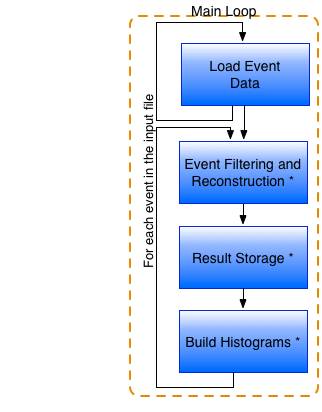
\includegraphics[scale=0.5]{imgs/new_loop.png}
		\caption{Schematic representation of the \textit{Main Loop} implementation modifications.}
		\label{fig:new_loop}
	\end{center}
\end{figure}

The interaction of the LipMiniAnalysis with the input data file is performed using the ROOT file reader classes. Since the event loading assumes also a set of operations, such as storing MonteCarlo information on \textit{EventData} and the \textit{FillAllVectors} initialisation, this task would benefit if it was executed in parallel, as the I/O itself only amounts to part of the computation. However, up to version ROOT v6, released in early June, it was not possible to have parallel file descriptors reading information of the same input file. With the new ROOT version it may be possible but it was not yet tested.

As previously stated, the \textit{DoCuts} function is responsible for filtering and reconstructing the events. The purpose of these filters is to separate the signal (interesting events) from the background (uninteresting events). The notion of an interesting event depends on the physics that the analysis studies, for example the background of a \ttH system analysis may contain events useful for the search of heavy quarks. As it may vary among different analysis, the \textit{DoCuts} must be coded by the user, but its structure is well defined. Implementation-wise, an analysis has a set of filters. Each filter is logically composed by a set of computations, more or less complex, and a test to the results of those computations. If the test fails, the event is not submitted to the rest of the filters. An example of a simple filter is to check if the mass of the event system (aggregate masses of all or a subset of particles detected) is greater than a given value, discarding events that do not provide interesting physics.

The reconstruction of an event is considered as a filter in \textit{DoCuts}, as only the events capable of being reconstructed pass the filter, which is usually the last. The reconstruction may be the most complex and computational intensive task in the whole data analysis application. One example is the \ttH system reconstruction, which performance depends on a trade-off between reconstruction accuracy and execution time. The event reconstruction is a task that may require a closer look to improve the efficiency of the data analysis, through a more specialised parallelisation on both homogeneous and heterogeneous platforms. Its irregular load and execution time, very complex algorithms, and few vectorised numerical computations creates a bottleneck complex to deal with, but with the potential of bringing exceptional performance gains when addressed with detail \cite{paperAMP}. Figure \ref{fig:new_docuts} presents a implemented prototype for a new \textit{DoCuts} flow that exposes the event reconstruction to more efficient parallelism approaches.

\begin{figure}[!htp]
	\begin{center}
		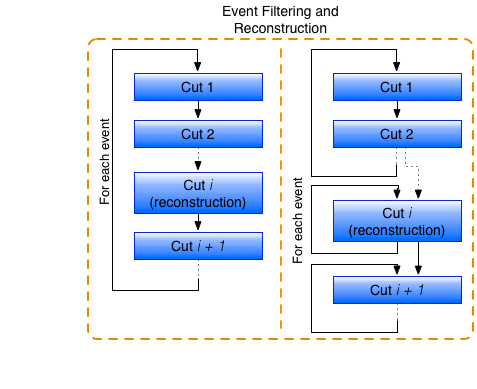
\includegraphics[scale=0.5]{imgs/new_docuts.png}
		\caption{Schematic representation current (left image) and proposed (right image) \textit{Event Filtering and Reconstruction} flows.}
		\label{fig:new_docuts}
	\end{center}
\end{figure}


Besides exposing the parallelism of a complex computational intensity section, this change also increases the workload to be simultaneously processed. When the application reaches the reconstruction, all events that passed the previous cuts can be processed in parallel. Having all the data necessary outside of the \textit{Main Loop}, as the \textit{Event Filtering and Reconstruction} as its own loop over all events on memory, but still hiding that fact from the user that codes \textit{DoCuts} to abstract the user as explained in \ref{new_framework}, allows for a better load balance of the possible parallelisation approaches, for homogeneous and heterogeneous platforms. For the latter, which operate in a distributed memory environment, it also helps to reduce the parallelisation overhead associated with the communications: instead of passing required the data of a single event multiple times, the data of all events is passed once. Then there is a third section of cuts (post-reconstruction) that are also coded by the user. To reduce the amount of loops, this third section shares the loop over all events with all the remaining post-processing of the \textit{Main Loop}. Note that both \textit{Main Loop} options will be available to maintain compatibility with the current data analysis applications.

\subsubsection*{Interfacing with legacy code}

Current data analysis use the data of an event as it is on the global memory, with no structure. The integration of the new event data structure requires that the accesses to the data be made through the STL collection used to store the event and the \textit{EventData} class. An interface is proposed to avoid rewriting the legacy code of these data analysis, a way to abstract the user from programming for a set of events by providing a kernel-like approach (where the code for processing an event is automatically applied to all). The interface must abstract both the access to the \textit{EventData} variables and methods, while being completely transparent to the user.

The input data files occasionally suffer some changes do to the increase in information given by the previous preprocessing on the CERN computational tiers. The file reading and the \textit{EventData} classes have to be adapted to this increase in event parameters. A static interface would need to be rewritten every time such change occurred. To avoid this problem, a parser was developed that receives the \textit{EventData} source files and retrieve the name of the methods and parameters. It then creates an header composed of \textit{define} clauses that translate the accesses to these variables on the STL collection to the previous simple accesses. This header is then included in the main LipMiniAnalysis header so that the user does not need to interact with the interface. This interface is automatically created every time the skeleton is compiled.

The user can code the data analysis assuming a single event is stored in memory. For example, to access an event luminosity the user would write \texttt{int var = LumiBlock}. However, when compiling the application the compiler preprocessor uses the interface to replace that statement with \texttt{int var = events.get(currentEvent).getLumiBlock()} without the user knowing how the event is stored. Note that the counter that assigns the event to process is automatically managed in every loop that iterates through the event data structure, hidden from the user.

\subsubsection*{Other features}

The final framework will have an utilities module where general features will be coded. Some of the already implemented range from automatic execution time measurement of the application and event processing throughput, definition of the number threads to execute, set the accuracy of some reconstructions. It was opted to use environment variables to set these features to reduce the clutter of options currently passed to the data analysis applications (usually more than 10 parameters) and separate general purpose features from physics functionalities.

One complex feature implemented is specific for the \ttH data analysis application. During the event reconstruction, several different variations of the system are reconstructed and only the best is of interest. For that a class was developed that encloses the resultant data of the reconstruction and performs a parallel merge through all the threads. This feature might prove useful for other data analysis once the structure of the class is general enough to hold the result of different types of reconstructions.
